\section{Einleitung}

Der heutige Netzwerkverkehr ist fast tausendfach größer als vor 20 Jahren \citep{Roser_I}. Das Internet wird heutzutage für fast all unsere Tätigkeiten verwendet: Soziale Netzwerke, Video und Audio-Streaming, Einkauf, behördliche Angelegenheiten und viele andere. So viel Verkehr generiert eine unermessliche Menge von Daten, die alle möglichen Inhalte beinhalten, von unschuldigen Anfragen nach einem eigenen Kontostand bis zur Ausführung von beabsichtigten Anfragen, um Systeme lahmzulegen. Um ersteres vom letzterem zu unterscheiden, verwenden viele Firmen das sogenannte \glsfirst*{SIEM} oder Log-Analyse-Tools. 

Das \glsfirst{NIST} definiert \gls{SIEM} als Software für die Sammlung, Anpassung, Analyse, Überwachung und Bedrohungserkennung von Sicherheitsdaten aus verschiedenen Quellen \citep{NIST_Definitions}. Die Bewertung dieser Daten spielt eine wesentliche Rolle bei solchen Anwendungen, um zu entscheiden, ob es sich um eine legitime Anfrage oder um einen \glsplural{Cyberangriff} handelt. Mit den Daten von \gls{SIEM} kann das \glsfirst{SOC} Team Maßnahmen ergreifen. Log Analysis und Log Management beziehen sich auf die Sammlung, Bearbeitung, Speicherung, Löschen, Weiterleitung und Überwachung von Loginformationen. In dieser Arbeit benutzen wir den Begriff \quotes{Log-Analyse-Tools}, um diese Systeme zu referenzieren.

In diesem Projekt recherchieren und vergleichen wir existierende \gls{SIEM} und Log-Analyse-Tools. Danach entscheiden wir uns für eine \gls{opensource} Lösung, um eine kostengünstige Verbreitung und Implementierung zu ermöglichen. Mit dem ausgewählten Tool analysieren und bewerten wir spezifische Logdateien, damit wir in Zukunft potenzielle Angriffe erkennen können. Die Regelsätze für die Angriffserkennung sollen mithilfe der \glsfirst{ttp} von \gls{mitre} aufgebaut werden.

\newpage
Unser Ziel ist es, eine umfangreiche \gls{opensource} Lösung zu finden bzw. zu gestalten, die uns ermöglicht, \glsplural{Cyberangriff} nach vordefinierten Regelsätzen zu detektieren. \glsplural{Proprietary} Lösungen gibt es viele auf dem Markt. Sie sind meistens kostenpflichtig und verlangen spezielle Wartung. Da sich solche Lösungen eher an große Konzerne richten, beschäftigen wir uns mit dem Aufbau und der Strukturierung einer eigenen Lösung mithilfe von \gls{opensource} Tools. 

Diese Arbeit wird in folgende Teile geteilt: 

% OSSIN: https://sourceforge.net/projects/os-sim/
% Preludes: https://www.prelude-siem.org/projects/prelude/wiki/ManualUser
% ELK Stack

% Grafana / Promtail: https://grafana.com/products/enterprise/
%https://grafana.com/logs/% 

%https://www.ossec.net/         https://github.com/ossec/ossec-rules

% was machen sie konkrent? / Vergleich zwischen OpenSource/Proprietary/

{\setstretch{1.5}
\begin{itemize}[noitemsep]
   \item	Definition von SIEMs und Log-Analyse-Tools 
   \item	Beschreibung von existierenden \gls{Proprietary}en und Open Source Lösungen
   \item	Entscheidung für die Implementierung von einer Open Source Lösung
   \item Generierung und Extrahierung von Logdateien nach der Ausführung von einem ausgewählten \gls{Cyberangriff} 
   \item	Installation, Konfiguration und Generierung von Warnmeldungen mit den ausgewählten Anwendungen 
   \item	Definition der \gls{usecases} und Implementierung der Regelsätze für die Erkennung der vorherigen Angriffe anhand der \glsfirst{ttp} der \gls{mitre} Matrix 
   \item	Auswertung der implementierten Tools mit der Verwendung von  spezifischen Logdateien der Hochschule in der ausgewählten Lösung
\end{itemize}
}

\subsection{Problemstellung}
Während der Entwicklung dieser Arbeit beschäftigen wir uns mit folgender Fragenstellung: 

{\setstretch{1.5}
% Regeln anhand mittre, automatisieren
\begin{itemize}[noitemsep]
   \item Wie können wir ein Log-Analyse-Tool konfigurieren, dass es vordefinierte Angriffe nach der \gls{mitre} Matrix automatisch erkennen kann? 
   \item Wie können wir allgemeine Regelsätze definieren, sodass wir sie später für die verschiedene \gls{ttp} der \gls{mitre} Matrix anpassen können?
\end{itemize}
}

\newpage
Das folgende Diagramm, \ref{fig:AblaufderArbeit}, stellt den Aufbau und Entwicklung dieser Arbeit dar, wie oben beschrieben:
% Diagram anpassen mit korrenkten Zielen

\begin{figure}[H]
   \centering
   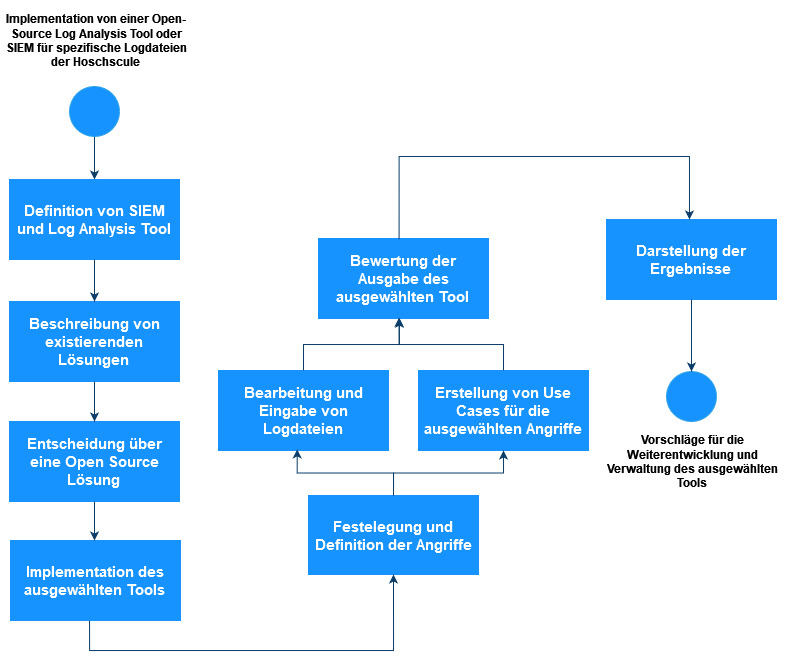
\includegraphics[width=1\textwidth]{assets/1_p1.jpg}
   \caption[Aufbau dieser wissenschaftlichen Recherche]
   {Aufbau dieser wissenschaftlichen Recherche \\Quelle: Eigene Darstellung }
   \label{fig:AblaufderArbeit}
   \centering
\end{figure}



